%===================================== CHAP 2 =================================

\chapter{Background Theory}

\section{Artificial Neural Networks}

\textit{This was missing in the specialization project. Need to cover all concepts used later in the report. This includes all different layers of a neural network. The layers (dropout, pooling, etc) could perhaps be a separate section after this one.}

\subsection{The Neuron}

Artificial Neural Networks (ANNs) are inspired by the structure and behavior of a biological brain, but they are generally not intended to be realistic models. A neural network consist of interconnected nodes referred to as units. These correspond to a biological neuron, the basic computational unit of the brain, structured as illustrated in \textbf{Fig. \ref{fig1}}. The connections between the units in an  corresponds to a biological neuron's dendrites, which provide input signals, and its single axon, which produces output signals and is connected to other neurons. \\

\begin{figure}
    \begin{minipage}{0.5\textwidth}
        \centering
            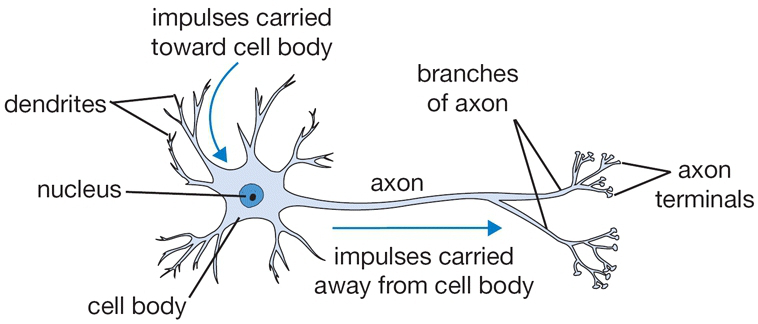
\includegraphics[width=1\textwidth]{fig/neuron}
            \caption{Biological neuron\cite{cs231n_part1}}
            \label{fig1}
    \end{minipage}
    \begin{minipage}{0.4\textwidth}
        \centering
            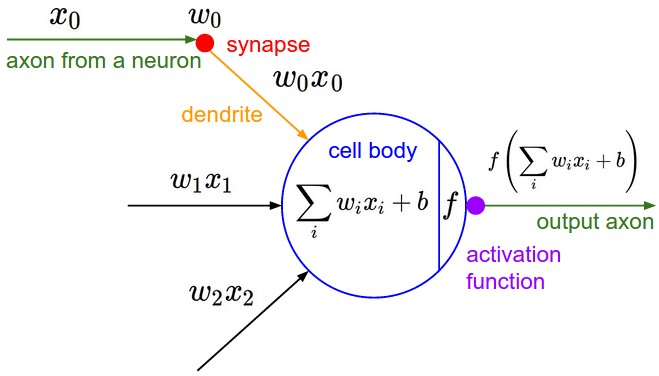
\includegraphics[width=1\textwidth]{fig/neuron_model}
            \caption{Mathematical model of a neuron\cite{cs231n_part1}}
            \label{fig2}
    \end{minipage}
\end{figure}

\noindent To simulate these signals, an ANN uses a mathematical model as illustrated in \textbf{Fig. \ref{fig2}}, where the signal is multiplied by the weight of a connection. The weight of a specific connection control how much the unit on one end influences the unit on the other end. The sum of all input signals are computed at the cell body of the unit. If this sum is above a certain threshold, the unit fires an output signal determined by its activation function by performing a specific mathematical operation on the sum.

\begin{itemize}
    \item The weights of a model can be learned by training the model on a set of input and output values.
    \item Perceptron? Outputs discrete 0 or 1 value vs sigmoid outputs smooth or continuous range of values between 0 and 1. Can also explain non-linearity.
    \item explain gradient descent and backpropagation.
\end{itemize}

\subsection{The Activation Function}

\noindent There are a great variety of activation functions in use, but we will only briefly describe those most commonly used and thus considered in our implementation. For further details we refer the reader to the Stanford CS class on convolutional neural networks\cite{cs231n_part1}. The common behaviour of all activation functions is that they define the output of a unit given a set of inputs. \\
\begin{figure}[H]
    \begin{minipage}{0.3\textwidth}
        \begin{tikzpicture}
            \begin{axis}[
                title = {Sigmoid function},
                axis lines = center,
                xtick={-10, -5, 5, 10},
                ytick={0, 0.2, 0.4, 0.6, 0.8, 1.0},
            ]
            \addplot [
                domain=-10:10,
                samples=100,
                color=blue,
            ]
            {1 / (1 + e^-x)};
            \end{axis}
        \end{tikzpicture}
    \end{minipage}
    \begin{minipage}{0.3\textwidth}
        \begin{tikzpicture}
            \begin{axis}[
                title = {Tanh function},
                axis lines = center,
                xtick={-10, -5, 5, 10},
                ytick={-1.0, -0.5, 0, 0.5, 1.0},
            ]
            \addplot [
                domain=-10:10,
                samples=100,
                color=blue,
            ]
            {(2 * (1 / (1 + e^-(2*x)))) - 1};
            \end{axis}
        \end{tikzpicture}
    \end{minipage}
    \begin{minipage}{0.3\textwidth}
        \begin{tikzpicture}
            \begin{axis}[
                title = {ReLU function},
                axis lines = center,
                xtick={-10, -5, 5, 10},
                ytick={2, 4, 6, 8, 1.0},
            ]
            \addplot [
                domain=-10:10,
                samples=100,
                color=blue,
            ]
            {max(0, x)};
            \end{axis}
        \end{tikzpicture}
    \end{minipage}
    \caption{Most common activation functions}
    \label{activationfuncs}
\end{figure}

\subsubsection{Sigmoid}

The sigmoid activation function is mathematically defined as $\sigma(x) = 1/(1 + e^{-x})$, plotted in \textbf{Fig. \ref{activationfuncs}}. The function takes a number as input, and outputs a number within a continuous range from 0 to 1. The sigmoid function has previously been used a lot, but because of its drawbacks, other activations functions tend to be preferred nowadays. The first drawback is that the outputs are not centered around zero, which can cause undesirable behaviour during gradient descent. A bigger drawback is that the activation saturates, meaning that the unit outputs mostly 0 and 1 instead of anything in between, and thus the gradient at these regions is very low. If the gradient falls to zero, the weights will not be updated through gradient descent, and so the network will stop learning.

\subsubsection{Tanh}

The tanh activation function is a scaled version of the sigmoid function. Its mathematical function, $tanh(x) = 2\sigma(2x) - 1$, is plotted in \textbf{Fig. \ref{activationfuncs}}. The scaling causes the tanh function to output numbers within the range of -1 and 1. This makes the output zero-centered, thus avoiding the first drawback of the sigmoid function. Even though the tanh function still stuffers from saturation, it is preferred to the sigmoid function.

\subsubsection{Rectified Linear Unit (ReLU)}

Describe the ReLU function.


\subsection{Optimizers/Loss Function}

\begin{itemize}
    \item SGD
    \item RMSprop
    \item Adagrad
    \item Adadelta
    \item Adam
    \item Adamax
    \item basically all optimizers keras provide, or only the ones we actually end up using
\end{itemize}

\subsection{Architecture}

\begin{itemize}
    \item Input and output layers
    \item Fully-connected layer
    \item Hidden layers
    \item Deep models
    \item Convolutional layer
    \item Dropout layer
    \item Pooling
\end{itemize}

\section{Convolutional Networks}

\textit{More in-depth than covered in the specialization project. \\
What exactly is the convolutional operation? Convolutional layer (local connections and weight sharing) vs normal layer.}

\section{Residual Networks}

\section{Face Recognition}

\textit{Can probably use a lot from the specialization project here.}

\section{Facial Expression}

\textit{Here as well.}

\section{Visualization}

\textit{Describe all the different techniques, perhaps in more detail. \\
Possibly even implementation level.}

\cleardoublepage